\section{Πρώτη Φάση Πειραμάτων}
\label{sec:experiments_phase1}

\subsection{AlexNet}

Οι παράμετροι των πειραμάτων είναι οι εξής:
\begin{itemize}
  \item{Αριθμός επαναλήψεων: 1000}
  \item{Αριθμός Νημάτων: 1, 2, 4, 8}
\end{itemize}

Στον \autoref{tab:alexnet_i7} παρουσιάζονται τα αποτελέσματα της μέσης τιμής
του χρόνου εκτέλεσης, ενώ στο \autoref{fig:alexnet_results_i7} φαίνεται
το διάγραμμα του χρόνου εκτέλεσης σε κάθε επανάληψη.

\begin{table}[H]
  \begin{center}
    \caption{Μετρήσεις πειραμάτων για το δίκτυο AlexNet σε επεξεργαστή Intel-i7-6700}
    \label{tab:alexnet_i7}
    \begin{tabular}{ | c | c | c | c | c | }
      \hline
      \rowcolor{Gray}
      \# νημάτων & 1 & 2 & 4 & 8 \\
      \hline
      Χρόνος εκτέλεσης (sec) & $0.117$ & $0.095$ & $0.095$ & $0.127$ \\
      \hline
    \end{tabular}
  \end{center}
\end{table}

Η μέγιστη τιμή μνήμης RAM που δεσμεύει το δίκτυο AlexNet μετρήθηκε στα \emph{692MB}.

\begin{figure}[H]
  \centering
  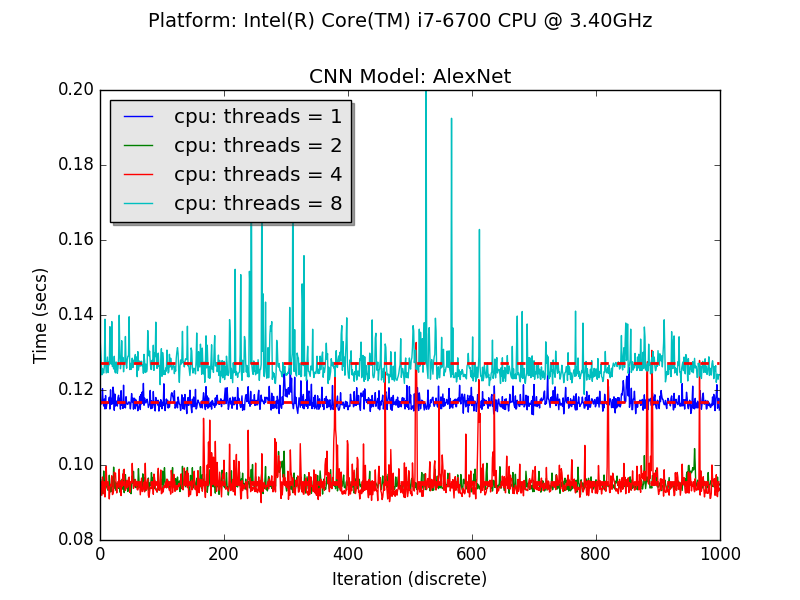
\includegraphics[width=0.8\textwidth]{./images/chapter6/benchmark_alexnet_i7.png}
  \caption[Χρόνoι εκτέλεσης για το δίκτυο AlexNet σε επεξεργαστή i7]{Χρόνοι εκτέλεσης για το δίκτυο AlexNet σε επεξεργαστή i7}
  \label{fig:alexnet_results_i7}
\end{figure}



%%----------------------------------------------------------------------------

\subsection{VGG16}

Οι παράμετροι των πειραμάτων είναι οι εξής:
\begin{itemize}
  \item{Αριθμός επαναλήψεων: 100}
  \item{Αριθμός Νημάτων: 1, 2, 4, 8}
\end{itemize}

Η μέσες τιμές του χρόνου εκτέλεσης των πειραμάτων παρουσιάζονται στον \autoref{tab:vgg16_i7}.
Η απαιτούμενη τιμή μνήμης RAM μετρήθηκε στα \emph{710MB}.

\begin{table}[H]
  \begin{center}
    \caption{Μετρήσεις πειραμάτων για το δίκτυο VGG16 σε επεξεργαστή Intel-i7-6700}
    \label{tab:vgg16_i7}
    \begin{tabular}{ | c | c | c | c | c | }
      \hline
      \rowcolor{Gray}
      \# νημάτων & 1 & 2 & 4 & 8 \\
      \hline
      Χρόνος εκτέλεσης (sec) & $0.7709$ & $0.5577$ & $0.4734$ & $0.6555$ \\
      \hline
    \end{tabular}
  \end{center}
\end{table}

\begin{figure}[H]
  \centering
  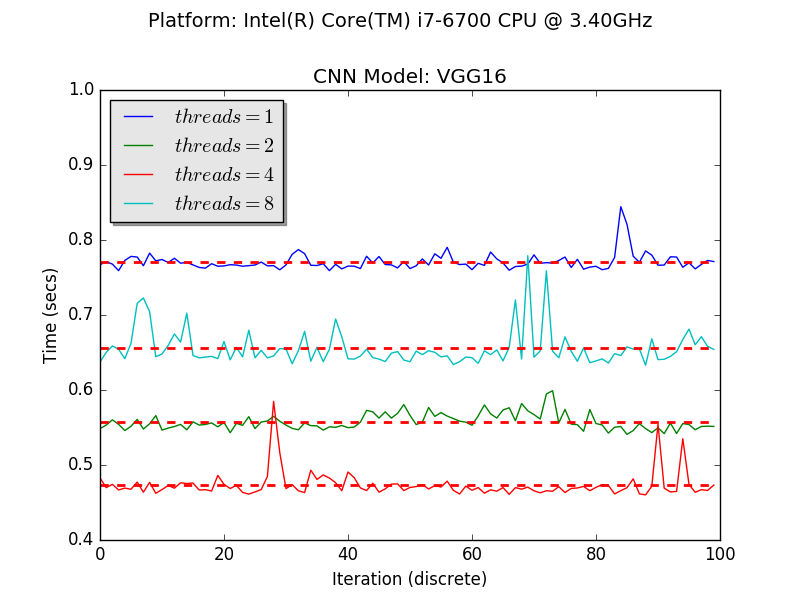
\includegraphics[width=0.8\textwidth]{./images/chapter6/benchmark_vgg16_i7.png}
  \caption[Χρόνoι εκτέλεσης για το δίκτυο VGG16 σε επεξεργαστή i7]{Χρόνοι εκτέλεσης για το δίκτυο VGG16 σε επεξεργαστή i7}
  \label{fig:vgg16_results_i7}
\end{figure}



%%----------------------------------------------------------------------------

\subsection{Tiny-YOLO}

Οι παράμετροι των πειραμάτων είναι οι εξής:
\begin{itemize}
  \item{Αριθμός επαναλήψεων: 1000}
  \item{Αριθμός Νημάτων: 1, 2, 4, 8}
\end{itemize}

Η αντίστοιχη μέση τιμή των χρόνων εκτέλεσης των πειραμάτων παρουσιάζονται στον \autoref{tab:yolo_i7}.
Σημαντικό να αναφερθεί ότι ο χρόνος εκτέλεσης της αντίστοιχης υλοποίησης της ερευνητικής ομάδας
που σχεδίασε το δίκτυο Tiny-YOLO, μετρήθηκε στα \emph{1.096 δευτερόλεπτα}.

\begin{table}[H]
  \begin{center}
    \caption{Μετρήσεις πειραμάτων για το δίκτυο Tiny-YOLO σε επεξεργαστή Intel-i7-6700}
    \label{tab:yolo_i7}
    \begin{tabular}{ | c | c | c | c | c | }
      \hline
      \rowcolor{Gray}
      \# νημάτων & 1 & 2 & 4 & 8 \\
      \hline
      Χρόνος εκτέλεσης (sec) & $0.18709$ & $0.1609$ & $0.1516$ & $0.2309$ \\
      \hline
    \end{tabular}
  \end{center}
\end{table}
Η μνήμη (μέγιστη) που απαιτείται κατά την διαδικασία
προς-τα-εμπρός εκτέλεσης μετρήθηκε στα \emph{379MB}.

\begin{figure}[H]
  \centering
  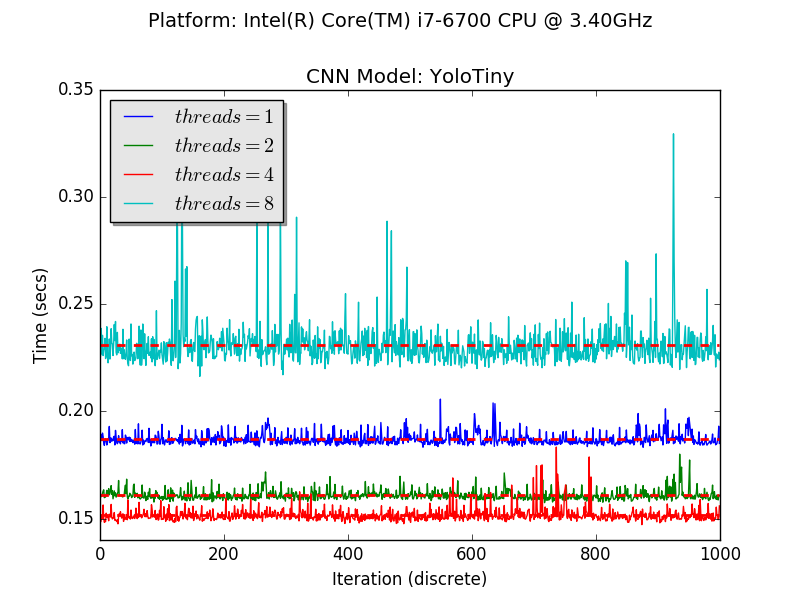
\includegraphics[width=0.8\textwidth]{./images/chapter6/benchmark_yolotiny_i7.png}
  \caption[Χρόνoι εκτέλεσης για το δίκτυο Tiny-YOLO σε επεξεργαστή i7]{Χρόνοι εκτέλεσης για το δίκτυο Tiny-YOLO σε επεξεργαστή i7}
  \label{fig:yolotiny_results_i7}
\end{figure}


